\chapter{空间金字塔分解的深度可视化方法}
\label{chap:visualization}

 提出了一种基于深度卷积神经网络自动识别超声心动图标准切面的方法,并可视化分析了深度模型的有效性。该算法针对网络全连接层占有模型大部分参数的缺点,引入空间金字塔均值池化替代全连接层,获得更多的空间结构信息,并大大减少模型参数、降低过拟合风险,通过类别显著性区域将类似注意力机制引入模型可视化过程。通过超声心动图标准切面的识别问题案例,试着对深度卷积神经网络模型的鲁棒性和有效性进行了解释。在超声心动图上的可视化分析实验表明,通过改进方法的深度模型的识别决策依据,同医师辨别分类超声心动图标准切面的依据一致,表明了方法的有效性和实用性。

\section{引言}

以深度卷积神经网络(Convolutional Neural Network ,CNN)为代表的深度学习对计算机视觉和机器学习领域产生了深远影响。但是完全理解深度学习模型的内在工作原理,设计高性能的深度网络结构还是很困难的,一直以来人们普遍将其内部工作原理看成一个“黑箱”,这是由于深度CNN存在海量参数,多次迭代更新生成输入输出之间相当不连续和非线性的映射函数;以及对参数的初始状态敏感,存在很多局部最优点。探究CNN的运行机制,核心在于它究竟自动提取什么样的特征,经过卷积层、池化层,特征都是分布式表达的,每个特征反映在原图上都会有重叠,故希望建立特征图与原图像之间的联系,即深度可视化。该技术试图寻找深度模型所提取各层特征较好的定性解释,并在设计开发新网络结构方面扮演重要角色。


目前针对CNN可视化的研究,主要集中在如何理解CNN从海量数据中自动学习到的,能反映图像本质的分层特征表达,即获得网络中隐藏层神经元与人类可解释性概念之间的联系。最直接的方法是展示学习得到的卷积核和相应的特征图,但除了首层卷积核和特征图有直观的解释外,其余各层并没有可解释性。从信号处理的角度看,基于CNN高层特征的分类器在输入域,需要较大感知野,才能对以由低频为主的输入图像进行多层非线性响应,并对小的输入改变产生平滑不变输出。同时,由于经过非线性激活函数变换和池化,引入空间不变性获得更好识别性能的同时,也对可视化带来新的挑战。


深度可视化技术可以简单分为三类:基于梯度更新的方法\citep{Erhan2009,simonyan14deep,Lenc2015,Szegedy2013a,JasonYosinski2015,Nguyen2016a,Nguyen2016b};基于特征重建的方法\citep{Zeiler2014,Brox,Mahendran2015d,Mahendran2015}];基于相关性的方法\citep{Cao2015,Bach2016}。基于网络梯度更新的思想是由Erhan等\citep{Erhan2009}引入,固定模型参数通过梯度更新改变输入值,最大化激活单一神经元或标签类别概率。激活最大化生成的非自然图像还可以是网络模型的对抗样本\citep{Goodfellow2014}。Simonyan等\citep{simonyan14deep,Lenc2015,Szegedy2013a}通过梯度上升方法迭代寻找使得最大化激活CNN某个或某些特定的神经元的最优图像,其假设神经元对像素的梯度描述了当前像素的改变能影响分类结果的强度。文献\citepns{simonyan14deep}引入L2正则化先验(或称权重衰减),改进可视化效果。Yosinski等\citep{JasonYosinski2015}进一步提出高斯模糊正则化、梯度剪切等技术,其中梯度剪切指的是每次只更新对分类最有利的一部分梯度,改善生成图像质量。文献\citepns{Lenc2015,Nguyen2016b}考虑神经元的多面性和利用生成网络作为自然图像的先验来合成更自然的图像。
Zeiler等\citep{Zeiler2014}提出利用反卷积网络,利用反向传播重构各层特征到像素空间的映射,并用于指导设计调优网络结构,提高分类识别精度。在反卷积过程中利用翻转原卷积核近似作为反卷积核,针对特定特征图在训练集上重新训练。Dosovitskiy等\citep{Brox}提出通过学习‘上’卷积网络来重建CNN各层的特征,指出结合强先验,即使用于分类的高层激活特征也包含颜色和轮廓信息。Mahendran等\citep{Mahendran2015d,Mahendran2015}通过对学习到的每层特征表达进行反编码重建,提出利用全变分正则化和自然图像先验,并将L2范数正则化推广到p范数正则化,得到较优的可视化效果。


本文主要关注前两种方法中的正则化技术,基于相关性分解方法请参考文献\citepns{Bach2016}。受文献\citep{Huang2017c,Denton2015}启发,把用于图像生成的拉普拉斯金字塔,进一步扩展成空间金字塔分解方法,并引入显著性激活图技术进一步改进深度CNN的可视化效果。
\section{可视化方法的数学模型}

激活最大化和特征表达反编码重建均是针对已经训练好的模型,对给定输入$x_{i}\in R^{C\times H\times W}$ ,其中C为颜色通道数,H,W为图像高和宽。CNN模型可抽象为函数$\phi$:$R^{C\times H\times W}\rightarrow R^d$ ,其第i个神经元的激活值为$\phi _{i}(x)$ ,对给定图像$x_{0}$ 的特征编码$\phi _{0}=\phi (x_{0})$ ,定义参数$\theta$ 的正则化项$R_{\theta}(x)$ ,寻找使得能量泛函最小化的初始输入$x^*$ ,其数学模型为
\begin{equation} \label{eq:ch04_01}
     x^*=\underset{x}{argmin} (l(\phi (x),\phi _{0})) + \lambda R_\theta(x))
\end{equation}
其中, $l$损失比较的是$\phi (x)$ 和目标$\phi_{0}$ 的差异,选择不同的损失函数定义不同的可视化方法。但该优化通常是一个非凸优化问题,通常采用梯度下降法去寻找局部最优值为
\begin{equation} \label{eq:ch04_02}
     x \leftarrow x+ \alpha \frac{\partial \phi _{i}(x)}{\partial x}
\end{equation}
激活最大化方法是文献\citepns{Erhan2009}中提出针对深度架构中任意层中的任意神经元所提取的特征,寻找使一个给定的隐含层单元的响应值$\phi _{0}\in R^d$ 最大的输入模式,可由内积形式定义$l$ 损失为
\begin{equation} \label{eq:ch04_03}
     l(\phi (x),\phi_{0}) =-<\phi (x),\phi _{0}>
\end{equation}
  式中$\phi_{0}$ 需人工指定,最大化激活的目标可以是全连接层的特征向量,也可以是卷积层某一通道的某一神经元的激活值。
特征表达的反编码重建,通过最小化给定特征向量与重建目标图像特征向量间的 损失,一般采用欧式距离来衡量损失误差,定义如下 
\begin{equation} \label{eq:ch04_04}
     l(\phi (x),\phi _{0}) = \frac{\parallel\phi (x)-\phi _{0} \parallel^2 }{\parallel \phi _{0} \parallel^2 }
\end{equation} 
但也可利用其它距离度量函数来评价损失。

\section{梯度更新的可视化方法}
 
   用于分类的深度CNN提取高层语义信息的同时,丢失了大量低层结构信息。由于首层卷积核大都类似Gabor滤波器,导致梯度更新可视化生成图像中包含许多高频信息,虽然能产生大的响应激活值,但对可视化来说导致生成的图像是不自然的。还由于网络模型的线性操作(如卷积)导致对抗样本\citep{Goodfellow2014}的存在,为得到更类似真实自然图像的可视化结果,需在优化目标函数中引入正则化作为先验。
\subsection{$p$ 范数正则化方法} 

   对图像来说,像素大小需在一定范围内,直接最大化激活类别概率,生成图像类似随机噪声图像。文献\citepns{simonyan14deep}通常引入L2范数正则化,惩罚过大和过小的极端值,其公式为$R_{\theta}(x)=\parallel x \parallel _{2}^{2}$ 。在文献\citep{Mahendran2015}中将其扩展到彩色图像RGB通道空间中的$p$范数正则化为
\begin{equation} \label{eq:ch04_05}
       R_{\theta}(x)= \frac{1}{HWC^p}\sum_{h=1}^{H}\sum_{w=1}^{W}(\sum_{c=1}^{C}x(x,w,c)^2)^{\frac{p}{2}}
\end{equation}
式中h,w表示图像的行和列大小,c表示颜色通道数,对比发现,文献\citepns{simonyan14deep}提出的L2正则化是忽视各颜色通道的差异的,正则化的力度可通过缩放常量p进行控制,即使得图像像素值大小保持在合适的范围内。
\subsection{高斯模糊和TV变分}

基于梯度更新可视化方法,引入高斯滤波器主动惩罚高频信息\citep{JasonYosinski2015},高斯模糊核半径大小由高斯函数的标准差控制,可随迭代次数动态调整模糊核大小。


全变分\citep{Mahendran2015}(Total Variance,TV)跟高斯模糊类似,鼓励可视化生成分片的常量块区域,对离散图像全变分操作可由有限差分来近似求解为    \begin{equation} \label{eq:ch04_06}
       R_{TV}(x)= \frac{1}{HWC^\beta}\sum _{hwc}((x(h,w+1,c)-x(h,w,c))^2+(x(h+1,w,c)-x(h,w,c))^2)^{\frac{\beta}{2}}
\end{equation}
式中 $\beta =1$,但其在可视化过程中,在图像的平坦区域并不存在边缘,全变分操作仍沿着边缘方向扩散就会导致出现虚假的边缘,会引入所谓的“阶梯效应”现象。 $\beta<1$时结合超拉普拉斯先验\citep{Krishnan2009}能更好匹配自然图像的梯度统计分布,但对可视化来说反而使得可视化更困难。文献\citepns{Mahendran2015}实际实验表明,跟高斯模糊核一样,需随迭代次数动态调整$\beta$ 大小。
\subsection{基于数据统计先验}

	由于常规可视化方法并没有对颜色分布进行建模,文献\citep{Lenc2015}提出通过引入外部自然图像数据,计算图像色块先验为
\begin{equation} \label{eq:ch04_07}
       R_{\theta}(x)= \sum_{p}\parallel x_{p}-D_{p}\parallel _{2}^{2}
\end{equation}
式中$p$为块索引,$x_{p}$ 表示稠密采样的归一化图像块, $D_{p}$表示自然图像块数据库中距离$x_{p}$ 最近图像块。该方法跟文献\citep{Huang2017c}中利用参考图像“指导”人脸图像嵌入重建类似。并且基于数据的统计先验可进一步扩展,引入生成对抗网络,利用生成网络主动生成自然图像先验\citep{Nguyen2016a}。

 
 
\section{空间金字塔分解}
 
前文介绍的正则化先验主动限制图像空间中高频率和高振幅信息,生成的可视化图像存在如下问题:1)彩色图像的颜色分布仍是不自然的。2)生成的图像中包含可识别类别对象的多个重复成分,并且这些部件不能组合成完整的有意义整体。3)缺乏令人可信的低频细节,存在棋盘效应,只是形似。针对这些问题提出利用空间金字塔分解,主动提升低频信息和调控高频信息以改善生成图像的可视化效果。

\subsection{高斯和拉普拉斯金字塔分解}
 
拉普拉斯金字塔(Laplacian Pyramid,LP)\citep{Burt1983}是由一系列包含带通滤波器在尺度可变的图像上加低频残差组成的。首先通过高斯平滑和亚采样获得多尺度图像,即第K层图像通过高斯模糊、下采样就可获得K+1层,反复迭代多次构建高斯金字塔(Gaussian Pyramid,GP)。用高斯金字塔的K层图像减去其第K+1层图像上采样并高斯卷积之后的预测图像,得到一系列的差值图像即为拉普拉斯金字塔分解图像。
拉普拉斯金字塔分解过程(见图1所示)包括4个步骤: 1)高斯平滑 ;2)降采样(减小尺寸); 3)上采样并高斯卷积(图中expand操作); 4)带通滤波(图像相减)  。拉普拉斯金字塔突出图像中的低频分量,拉普拉斯金字塔分解的目的是将源图像分解到不同的空间频带上。
\begin{figure}[!htbp]
\centering
%trim option's parameter order: left bottom right top
%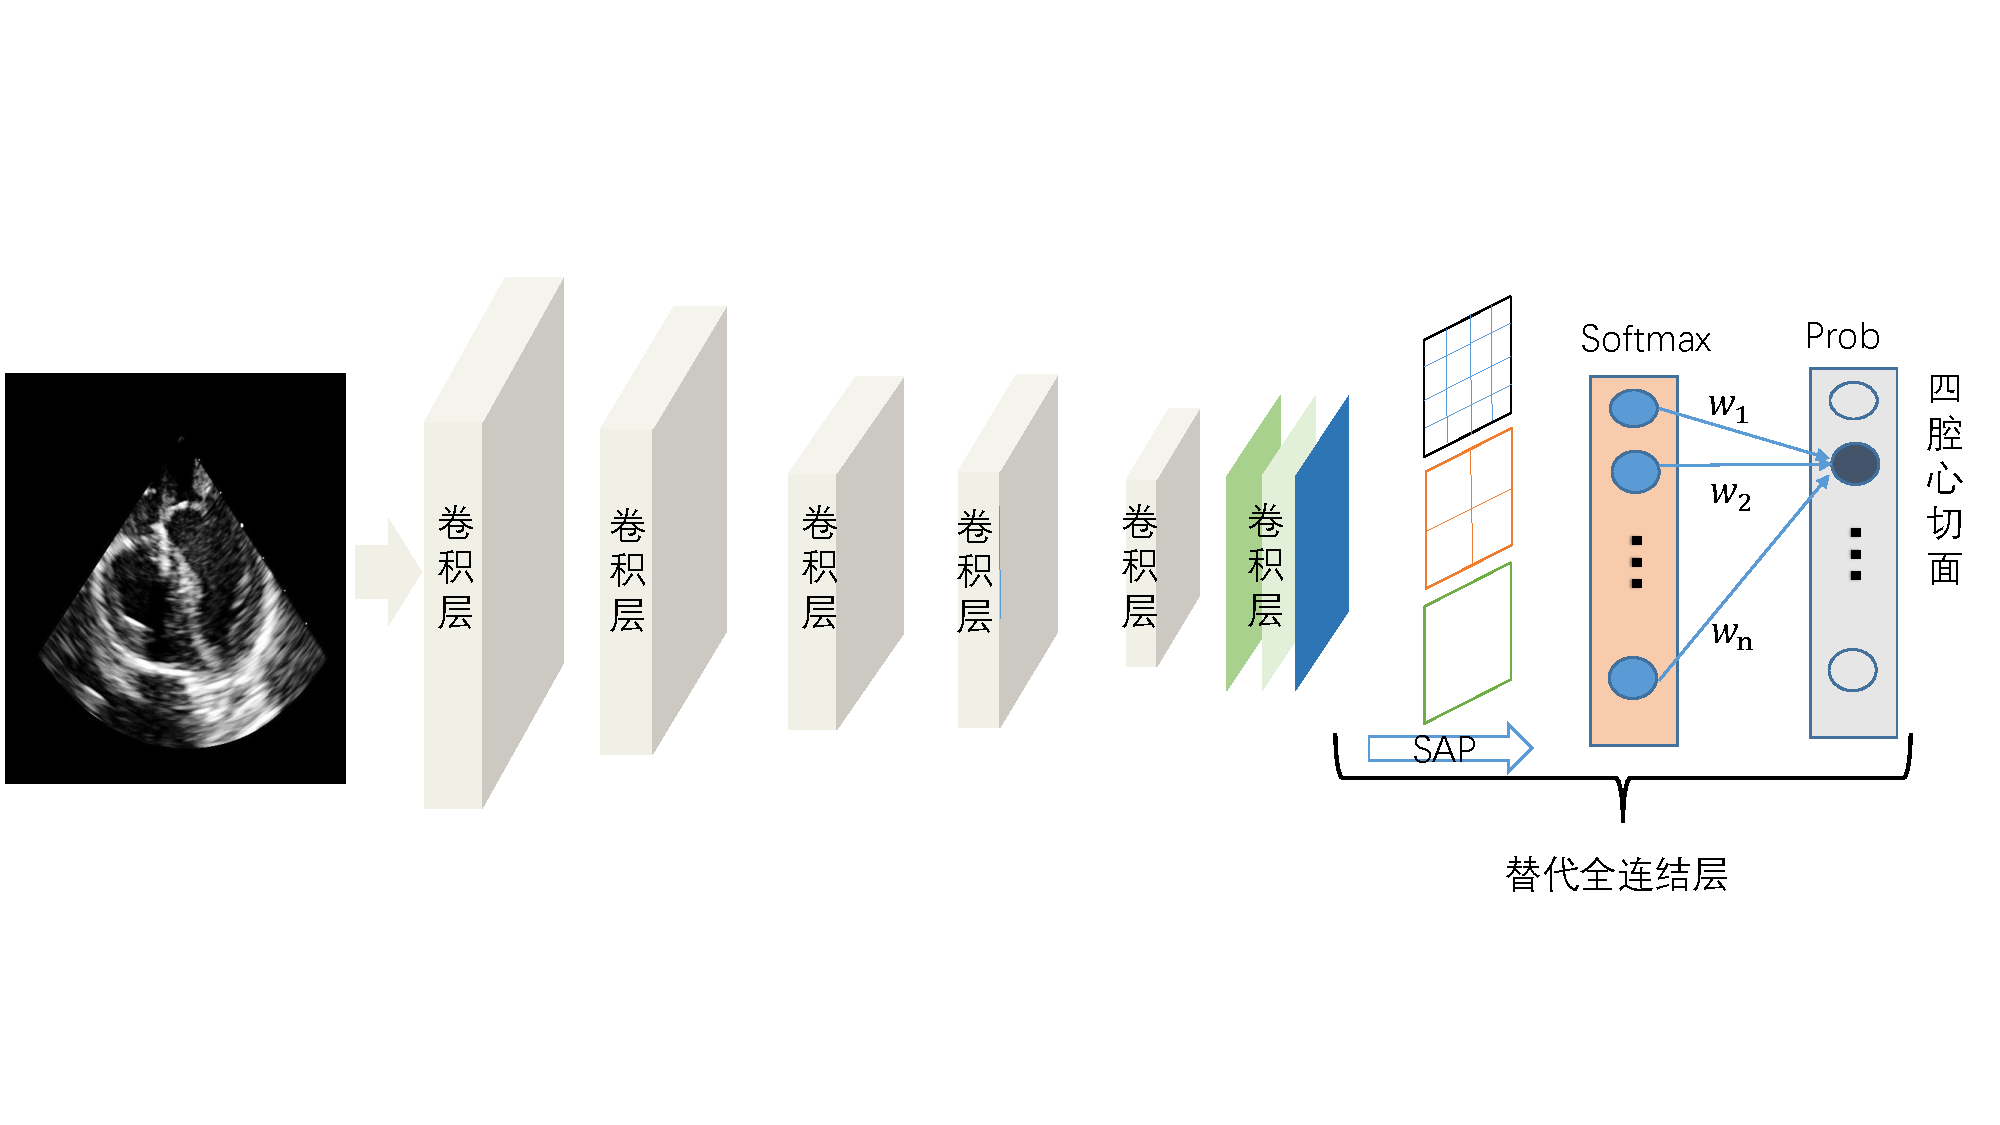
\includegraphics[trim = 30mm 0mm 30mm 0mm, clip, width=0.45\textwidth]{ch03_02}
\includegraphics[width=0.85\textwidth]{ch04_01}
\caption{高斯和拉普拉斯金字塔}
\label{fig:ch04_01}
\end{figure}

	由于自然图像统计特性中的尺度不变性,也称为$1/f$法则\citep{VanderSchaaf1996a},即自然图像集$I(f_{x},f_{y})$ 的平均傅里叶功谱服从$I~(f_{x},f_{y})^2$ 。在激活最大化可视化深度CNN模型过程中利用提出的高斯和拉普拉斯空间金字塔分解,调整生成梯度图像包含的频谱分量大小。其中空间金字塔分解正则化项为
\begin{equation} \label{eq:ch04_08}
       r_{\theta}(x)= \sum_{k=1}^{K}[LP_{k}+GP_{k}]
\end{equation}
式中k代表构建$k$层金字塔分解,本文实验$k$选取为4。 $LP_{k}$为第$k$层的拉普拉斯金字塔分量,$GP_{k}$ 为第$k$层的高斯金字塔分量。 


\subsection{梯度归一化}
  
	基于梯度更新的可视化方法,由于原输入空间中高低频分量混杂在一起,对原输入图像相应的更新梯度进行归一化操作能得到较好可视化效果,即对输入图像每次迭代更新的梯度 ,则提出梯度归一化操作:   
\begin{equation} \label{eq:ch04_09}
       g \rightarrow \frac{g}{g.std()+\delta}
\end{equation} 
式中 $\delta$为非负小常量,std表示梯度矩阵的方差。该梯度中心归一化技术,可以减少产生重复的对象碎片的倾向,而倾向于产生一个相对完整对象。梯度归一化的引入同批归一化(Batch Normalization)思想类似,校正CNN网络非线性变换引起的“偏移”,该方法也侧面验证最新提出的分层归一化\citep{Ioffe2014}的有效性。
\subsection{类别激活图限制可视化区域}
根据文献\citepns{Zhou2015}提出的类别激活图技术,假设$f_{j}(x,y)$  表示最后的卷积层空间$(x,y)$位置上第$j$ 个神经元的激活值,则对$j$ 神经元的全局平均池化操作结果对给定类别$k$的得分函数$S_{k}$:
\begin{equation} \label{eq:ch04_10}
      S_{k}=\sum _{j} w_{j}^{k} \sum _{x,y}f_{j}(x,y)
\end{equation}
式中 $w_{j}^{k}$ 是第$j$ 个神经元和第 k类的连接权重。根据文献\citepns{Zhou2015},由式\ref{eq:ch04_10} 可得定义类别激活图$M_{k}$ 为	
\begin{equation} \label{eq:ch04_11}
      M_{k}=\sum _{j} w_{j}^{k}f_{j}(x,y)
\end{equation}
式中$M_{k}$ 表明在空间(x,y)位置的激活值对分类结果影响的重要性。对类别激活映射图直接双线性插值得到与原输入图像大小相等的显著性图。本文利用显著性激活图作为梯度更新的权重因子,即输入变为原始输入图像与类别激活图的加权乘积。动机是要求网络梯度更新保持在类别显著性区域内,压制无关背景信息的生成。具体详情请参见第四章实验部分。
\subsection{优化方法}

深度CNN模型优化策略的核心是随机梯度下降法,常用方法是带动量的随机梯度下降法为:
\begin{equation} \label{eq:ch04_12}
      V_{t}=\mu V_{t-1} -\alpha *\bigtriangledown {f(x_{i})}
\end{equation}          
\begin{equation} \label{eq:ch04_13}
     x_{t+1}=x_{t}+V_{t}
\end{equation}       
式中$\mu$ 为动量因子表示保持原更新方向的大小,一般选取0.9, $x_{t}$为在t时刻待更新的梯度,$\alpha$ 为学习率;文献\citep{Mahendran2015d,Mahendran2015} 采用自适应梯度(Adaptive Gradient,AdaGrad)\citep{Duchi2011}的变种算法,根据历史梯度信息自适应调整学习率。同时文献\citepns{Gatys2015a}采用的二阶优化算法针对纹理和艺术风格重建问题,得到比用基于一阶随机梯度下降算法更优的可视化效果。但本文通过实验对比发现对各种优化方法对生成图像质量影响不大,从简选择带动量的随机梯度优化方法。
\section{实验结果分析和讨论}
 
基于梯度更新的可视化方法主要用于激活最大化和特征重建,但文献\citepns{He2016}指出用随机未训练的CNN模型也能较好重建原图像,表明特征编码重建不能很好解释训练得到CNN模型的内在工作机理。故本文实验主要关注在对ImageNet公开数据集上预先训练得到的分类模型进行激活最大化可视化实验。

\subsubsection{不同深度模型的类别可视化} 
\begin{figure}[!htbp]
\centering
%trim option's parameter order: left bottom right top
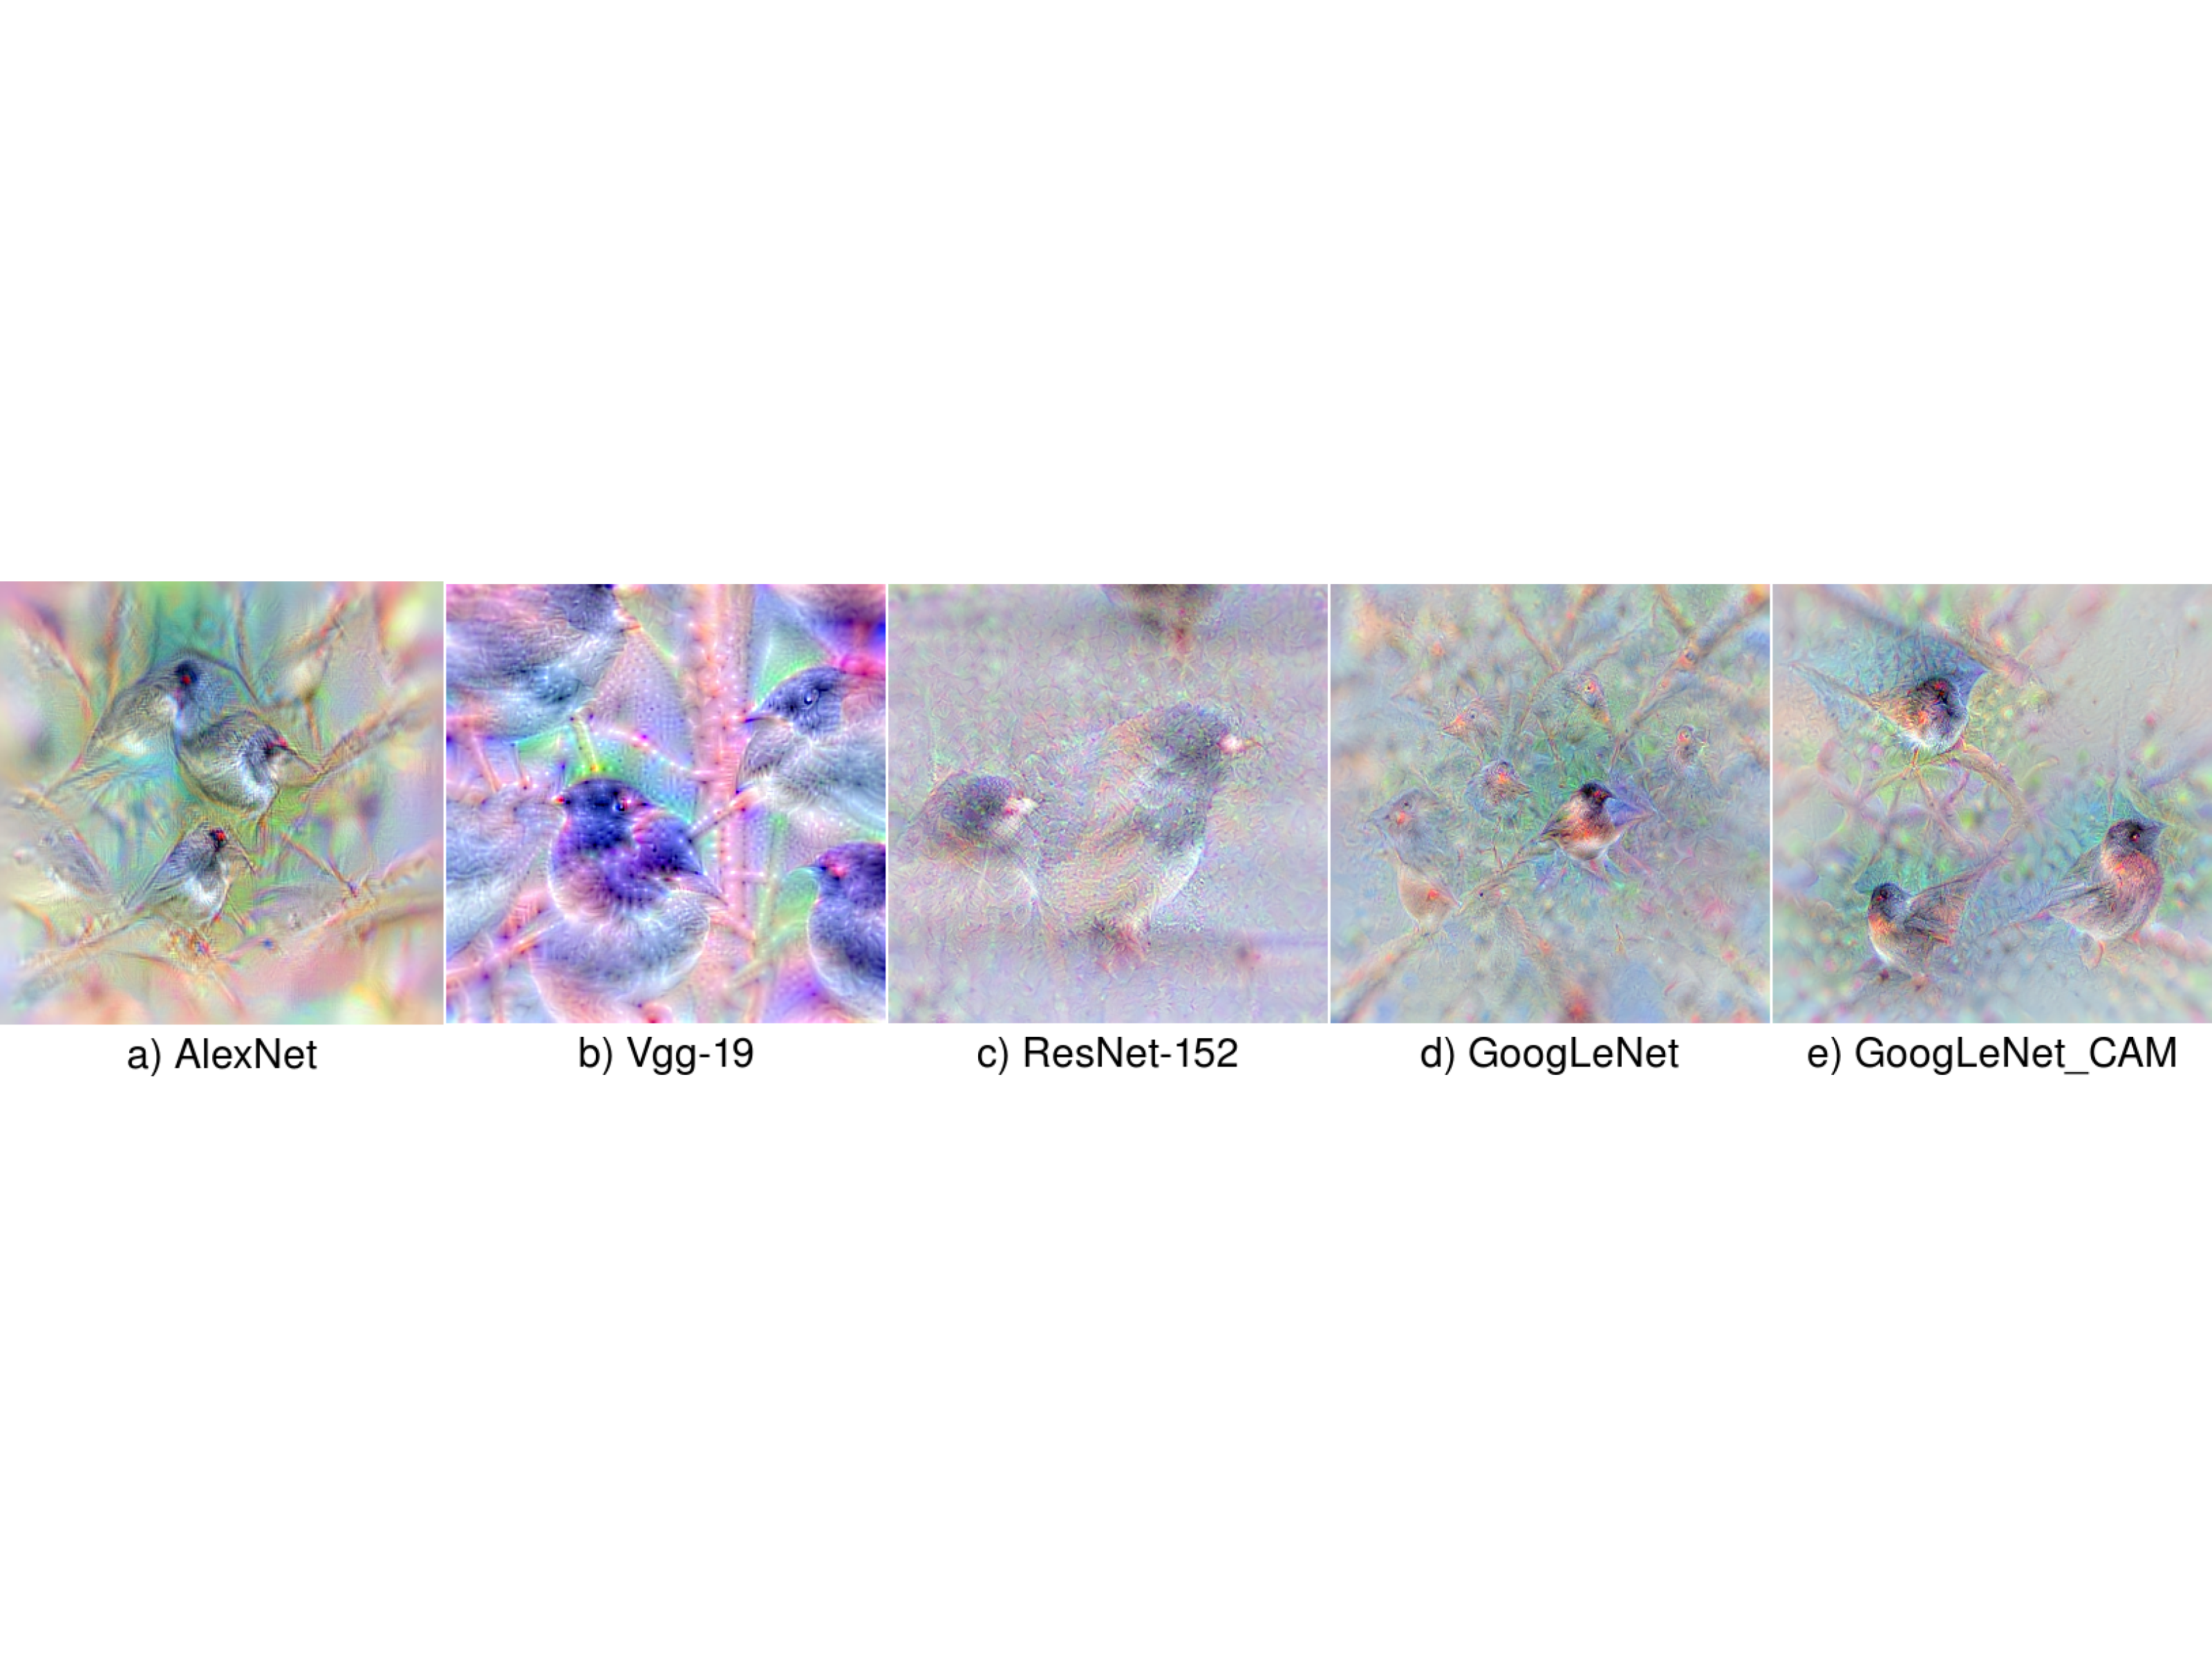
\includegraphics[trim = 0mm 35mm 00mm 35mm, clip, width=0.85\textwidth]{ch04_02}
%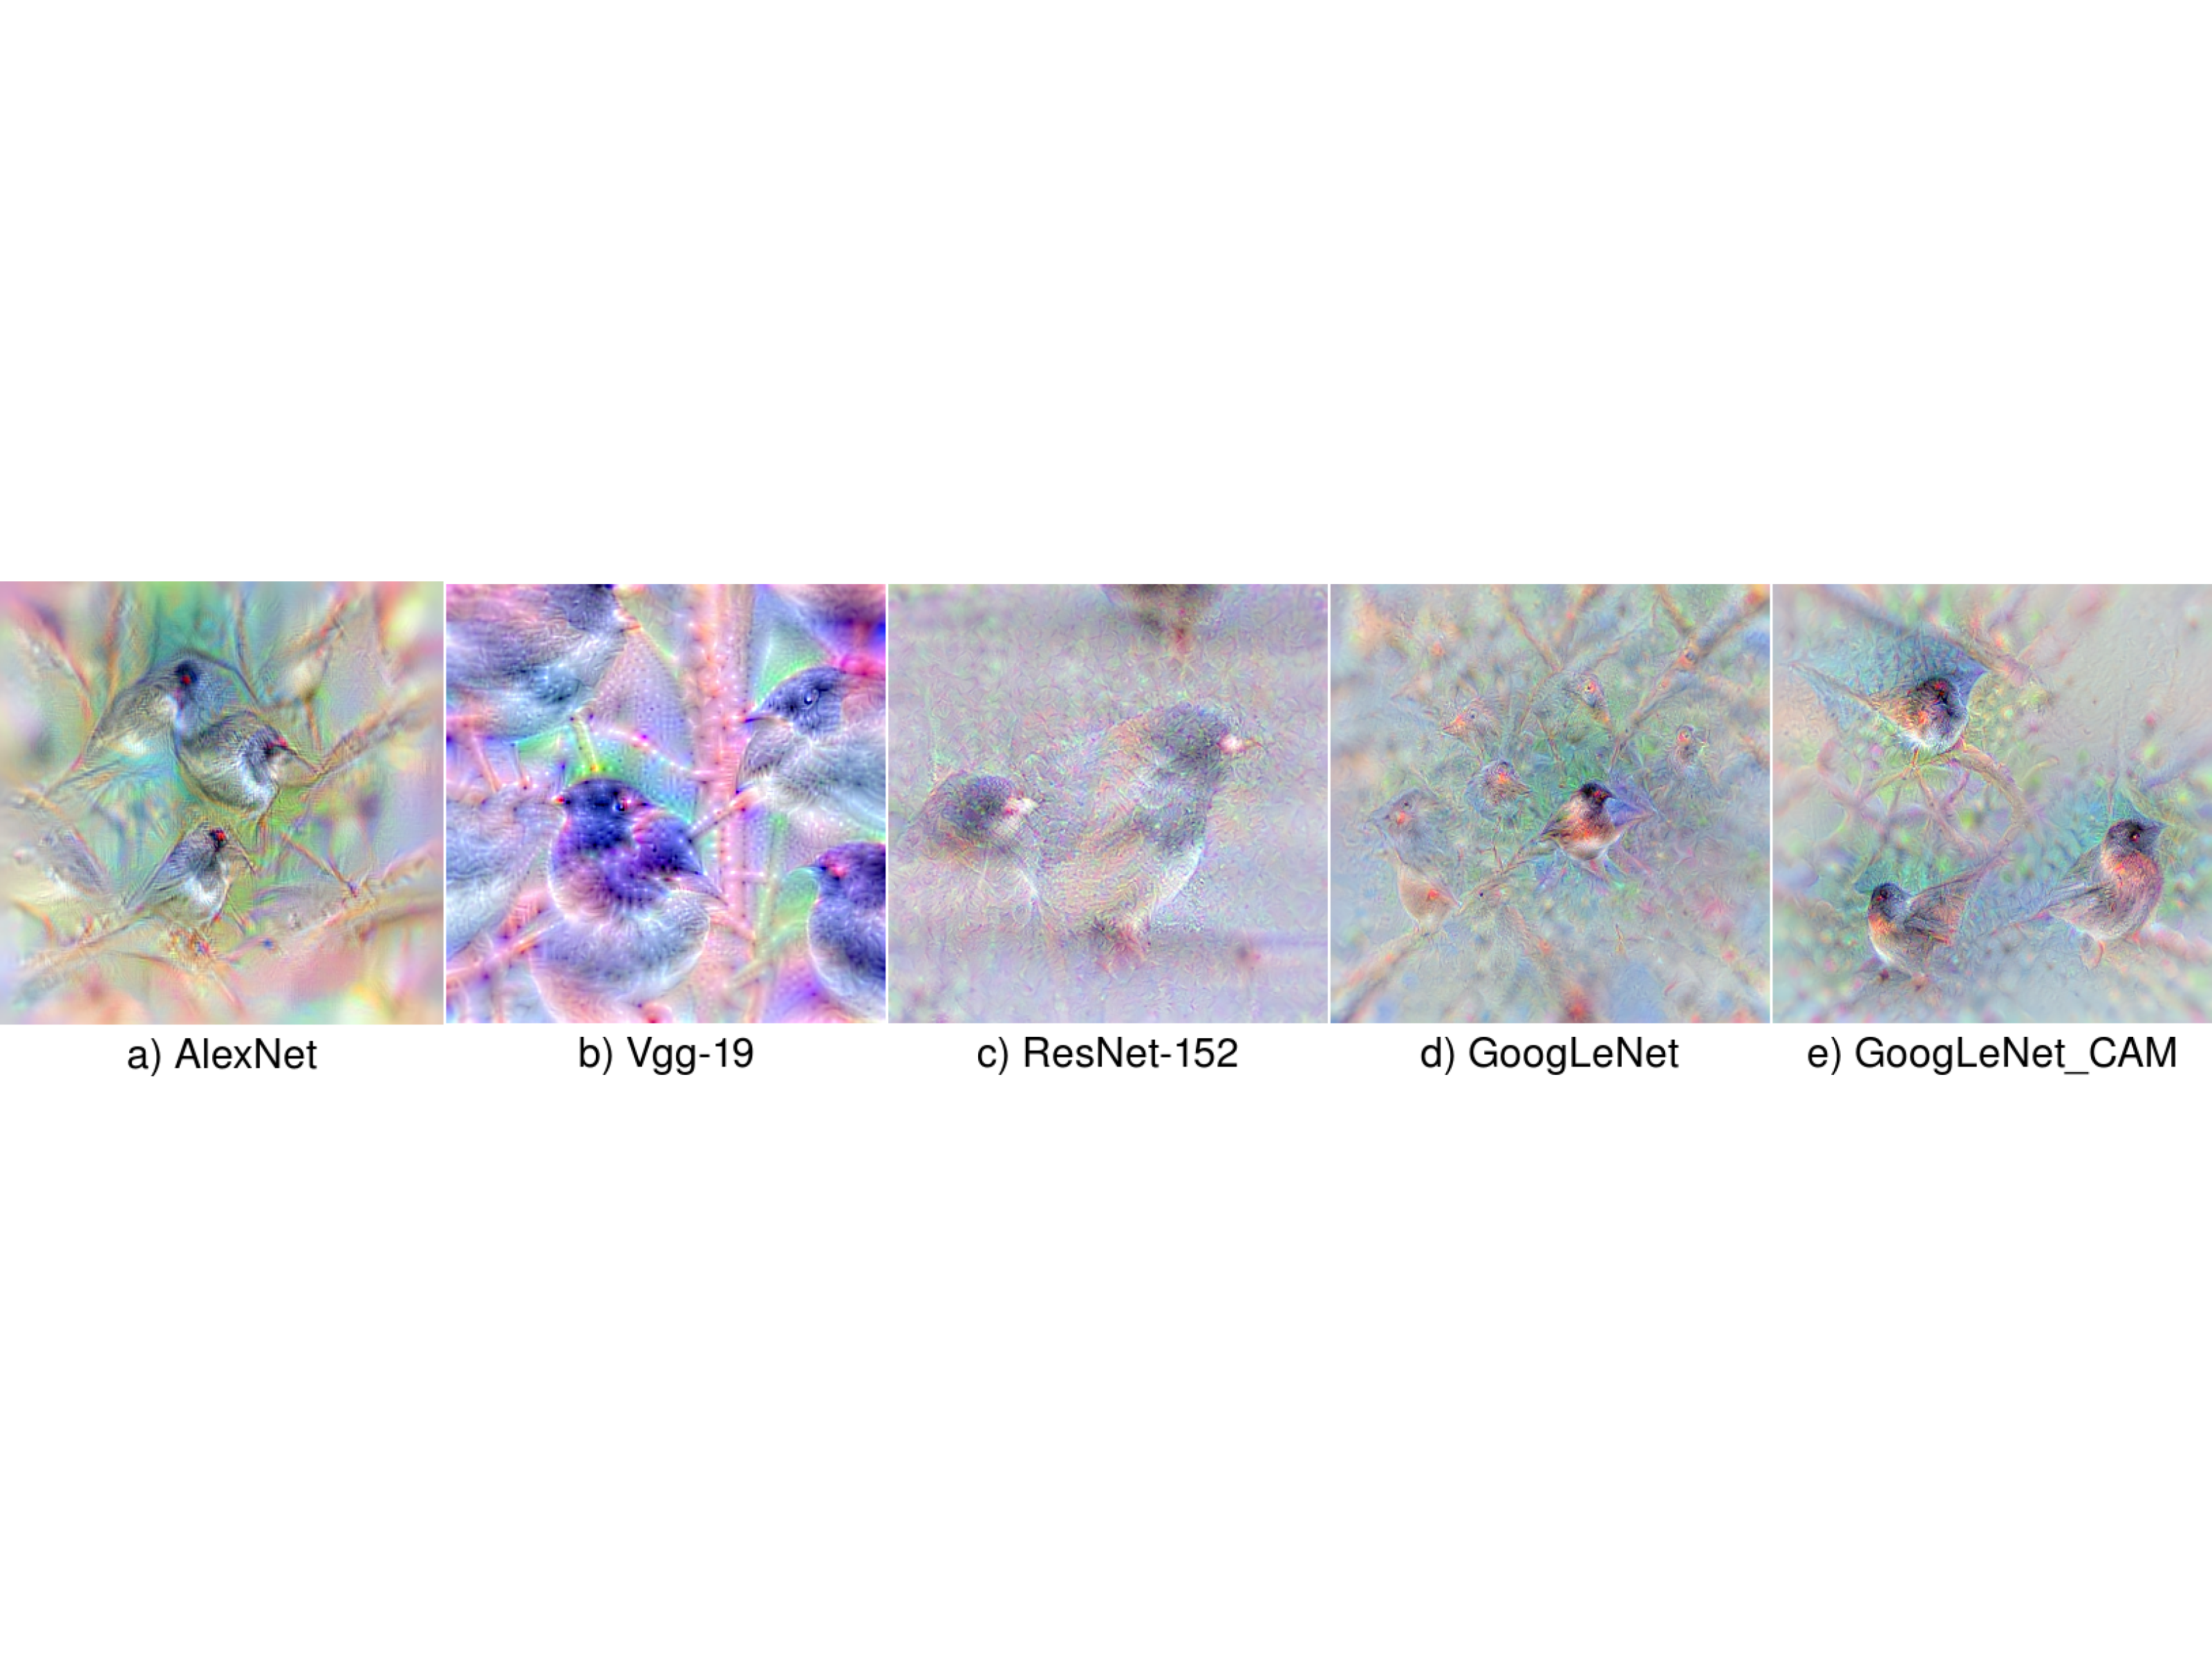
\includegraphics[width=0.85\textwidth]{ch04_02}
\caption{不同模型类别可视化实验结果}
\label{fig:ch04_02}
\end{figure}

实验选取的深度模型来自于开源社区的Caffe model zoo,不同的CNN模型如:AlexNet模型\citep{Krizhevsky2012},Vgg-19模型\citep{Simonyan2014a},Google-CAM模型\citep{Zhou2015},GoogleNet模型\citep{Szegedy2015},ResNet模型\citep{he15},其分类识别性能依次从低到高,模型的复杂程度依次递增。本文实验默认采用提出的梯度归一化,并引入多分辨率、随机扰动和剪切等小技巧作为通用设置,提高可视化效果。


为比较不同深度CNN模型学习相同类别时特征图的差异,根据式\ref{eq:ch04_01},给定高斯噪声生成随机图像作为输入,指定可视化物体类别向量(见图\ref{fig:ch04_02}所示,类别为所有类别中的第13类布谷鸟),施加前文提出不同正则化项的组合:p范数、高斯模糊和金字塔分解正则化。


图\ref{fig:ch04_02}结果表示5种CNN模型在相同正则化方法和相同梯度更新策略下的可视化效果,对比图\ref{fig:ch04_02}中a,b,c发现随着网络模型深度的增加,可视化难度增大分类性能同可视化效果一致;Vgg-19模型由于跟ResNet模型卷积核大小类似,且比AlexNet首层卷积核小(7和3),即可视化效果倾向生成比AlexNet更大尺寸的物体。而由图\ref{fig:ch04_02}中a,d,e对比可知,由于GoogleNet模型中卷积层的卷积核大小不一,使得可视化结果中引入更多细节。综合可知,基于GoogleNet模型的可视化效果最好,后面实验均是在其模型的基础上进行实验比较。

\subsubsection{ 不同正则化方法的类别可视化}
为验证不同正则化方法对理解深度模型的特征表达的影响,采取前文所述的不同正则化方法,可视化效果结果见图\ref{fig:ch04_03}所示,从上到下依次可视化类别为金甲虫,海星,蝎子,酒壶,卷笔刀。
 
\begin{figure}[!htbp]
\centering
%trim option's parameter order: left bottom right top
%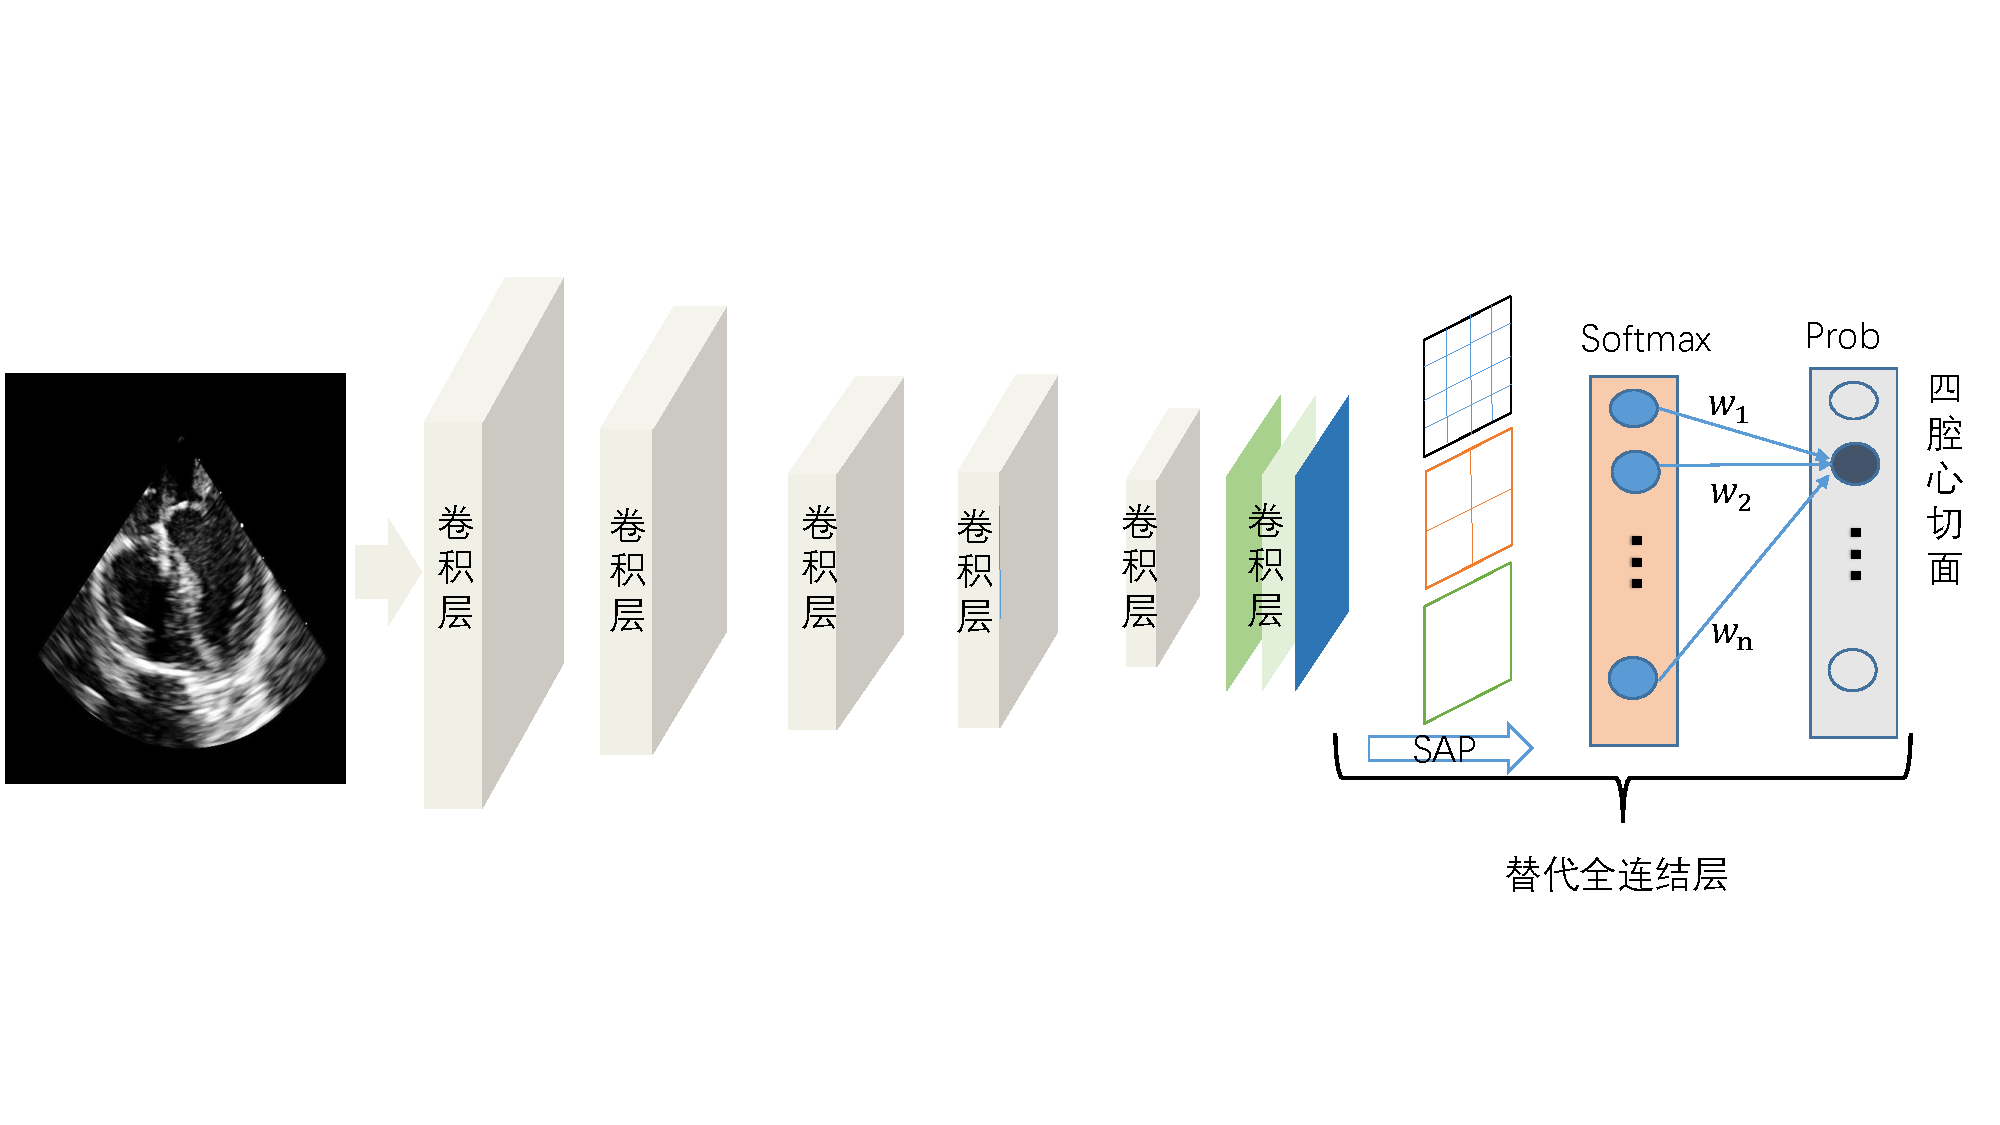
\includegraphics[trim = 30mm 0mm 30mm 0mm, clip, width=0.45\textwidth]{ch03_02}
\includegraphics[width=0.85\textwidth,height=0.4\textheight]{ch04_03}
\caption{不同正则化方法的可视化效果}
\label{fig:ch04_03}
\end{figure}

图\ref{fig:ch04_03}中(a)列仅施加默认设置和不加梯度归一化的结果,由于输入的随机性,并不能保证每次都生成有意义的可视化结果,但引入本文提出的梯度归一化后,能大概率生成可视化结果见图\ref{fig:ch04_03}(b)列所示,图\ref{fig:ch04_03}(c)列表示只采用p范数正则化,跟文献\citep{•}2]一致取2,使得图像更平滑,但仍与真实图像相差较大。通过前文理论分析和实验验证,全变分跟高斯模糊作用类似,本文采用根据迭代轮数动态调整高斯模糊核大小,具体是在刚开始采用较大值希望生成物体大概轮廓,随迭代逐渐调小模糊核使得更多细节生成,具体见图\ref{fig:ch04_03}(d)。但是这个参数无法自适应设置为最优,对图像高低频分量无法调整控制,而本文提出的利用金字塔分解正则化方法能从粗到细调整,产生较优结果见图\ref{fig:ch04_03}(e)列所示。
\subsection{金字塔分解可视化实验结果}

为验证提出金字塔分解正则化方法,对中间层卷积核的可视化,采用前文提出式\ref{eq:ch04_08},指定深度CNN模型中不同卷积层中不同通道,利用前文提出的带动量的梯度更新策略,可视化结果见图\ref{fig:ch04_04},其中从上到下依次为GoogleNet模型低中高层不同通道的可视化结果,与文献\citep{Zeiler2014}一致,低层多尺度分辨率生成的纹理见图\ref{fig:ch04_04}首行所示,中层是一些物体部件,见图4中间行所示蜜蜂的局部结构,而高层是更完整的抽象概念见图\ref{fig:ch04_04}下层中完整的花瓣。对比图\ref{fig:ch04_04}(b)、(c)列,可验证拉普拉斯金字塔主动分解提升图像部分低频成分,而高斯金字塔分解生成的图像中高频细节更突出。
\begin{figure}[!htbp]
\centering
%trim option's parameter order: left bottom right top
%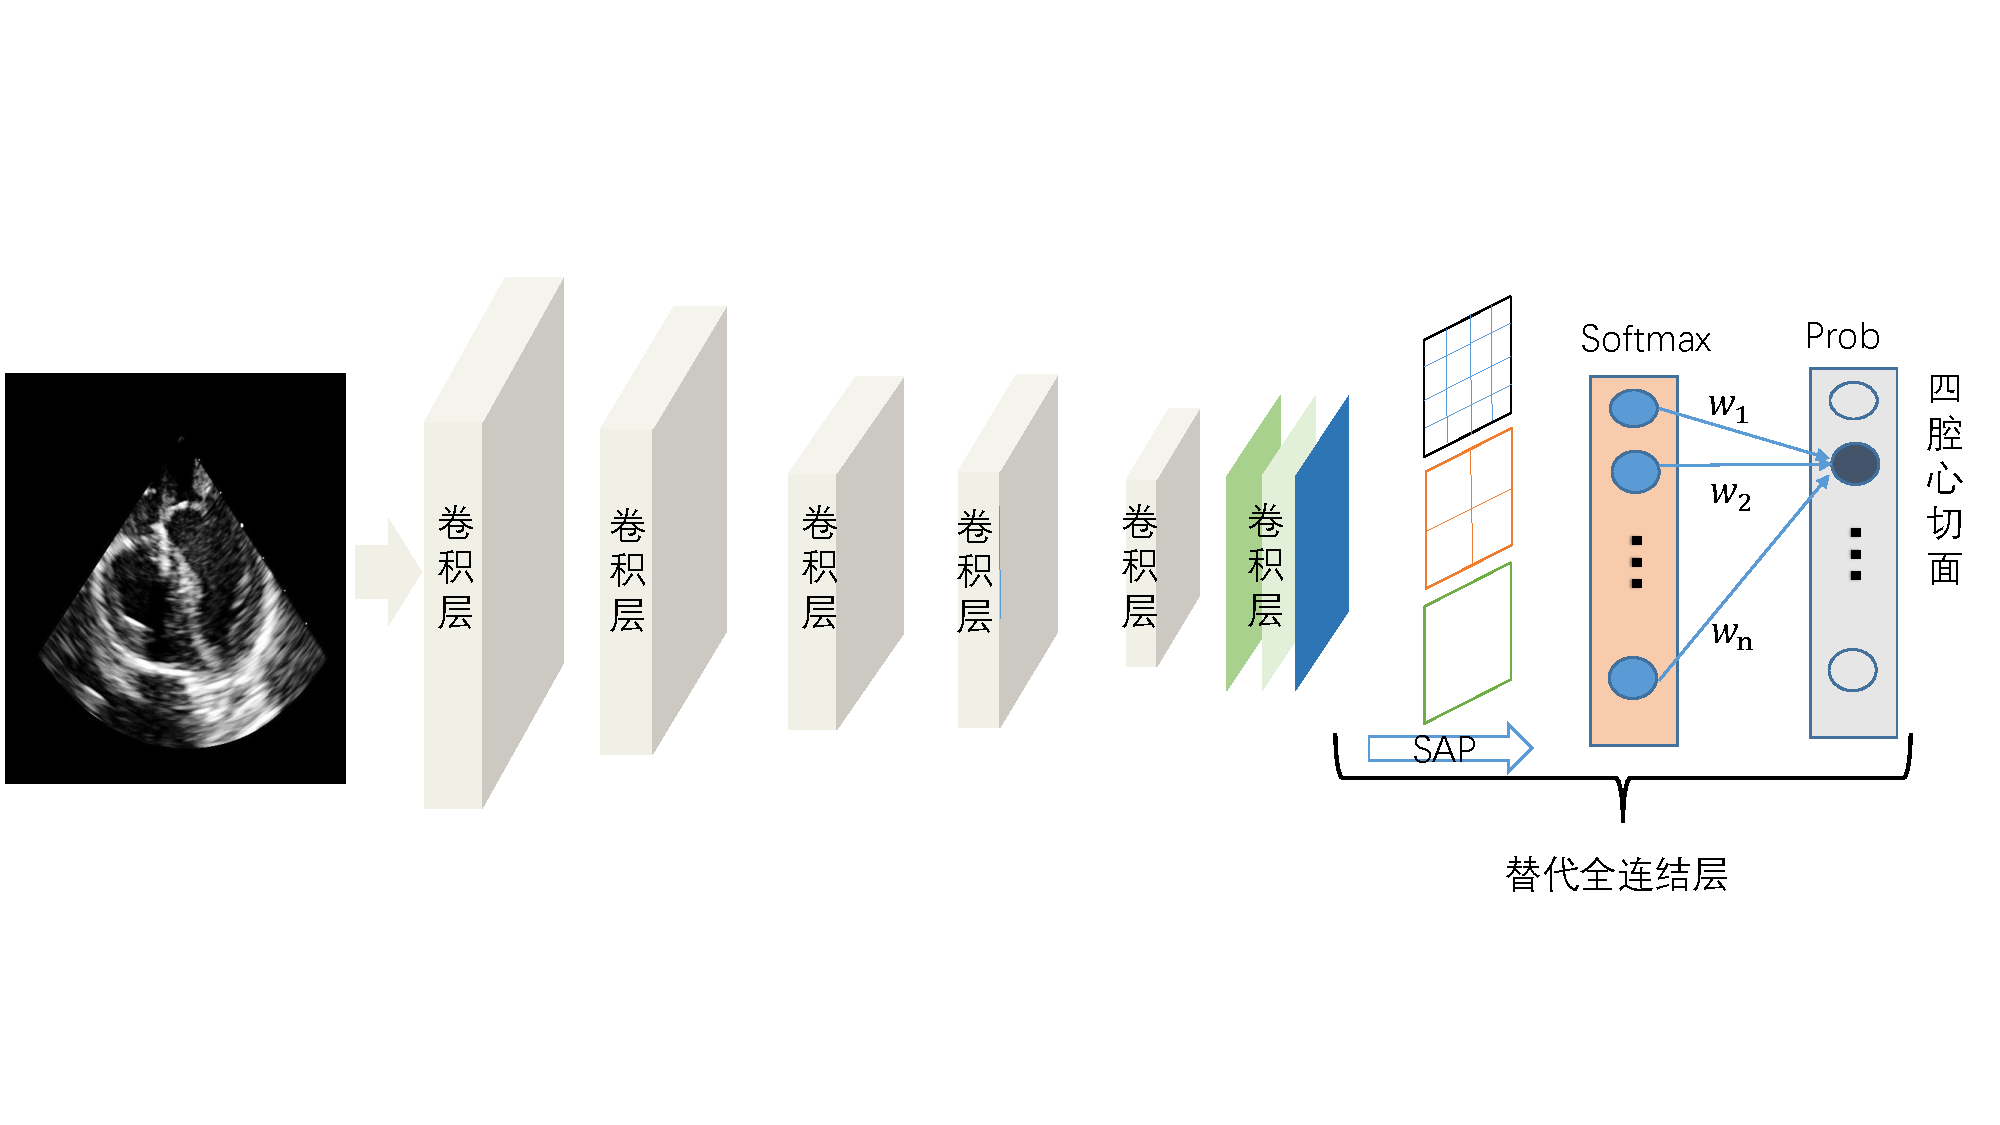
\includegraphics[trim = 30mm 0mm 30mm 0mm, clip, width=0.45\textwidth]{ch03_02}
\includegraphics[width=0.85\textwidth,,height=0.4\textheight]{ch04_04}
\caption{金字塔分解正则化可视化效果}
\label{fig:ch04_04}
\end{figure} 

\subsection{引入类别显著性的可视化} 

通过观察之前可视化结果可知,生成的图像中除了该类别外仍有许多额外的上下文信息(见图\ref{fig:ch04_02}中鸟类别的树枝),这些信息与模型的分类能力相关联,可通过引入类别激活图可改善可视化效果。迭代更新过程中依据采用式\ref{eq:ch04_11},使用类别激活图作为加权因子限制迭代更新区域。
\begin{figure}[!htbp]
\centering
%trim option's parameter order: left bottom right top
%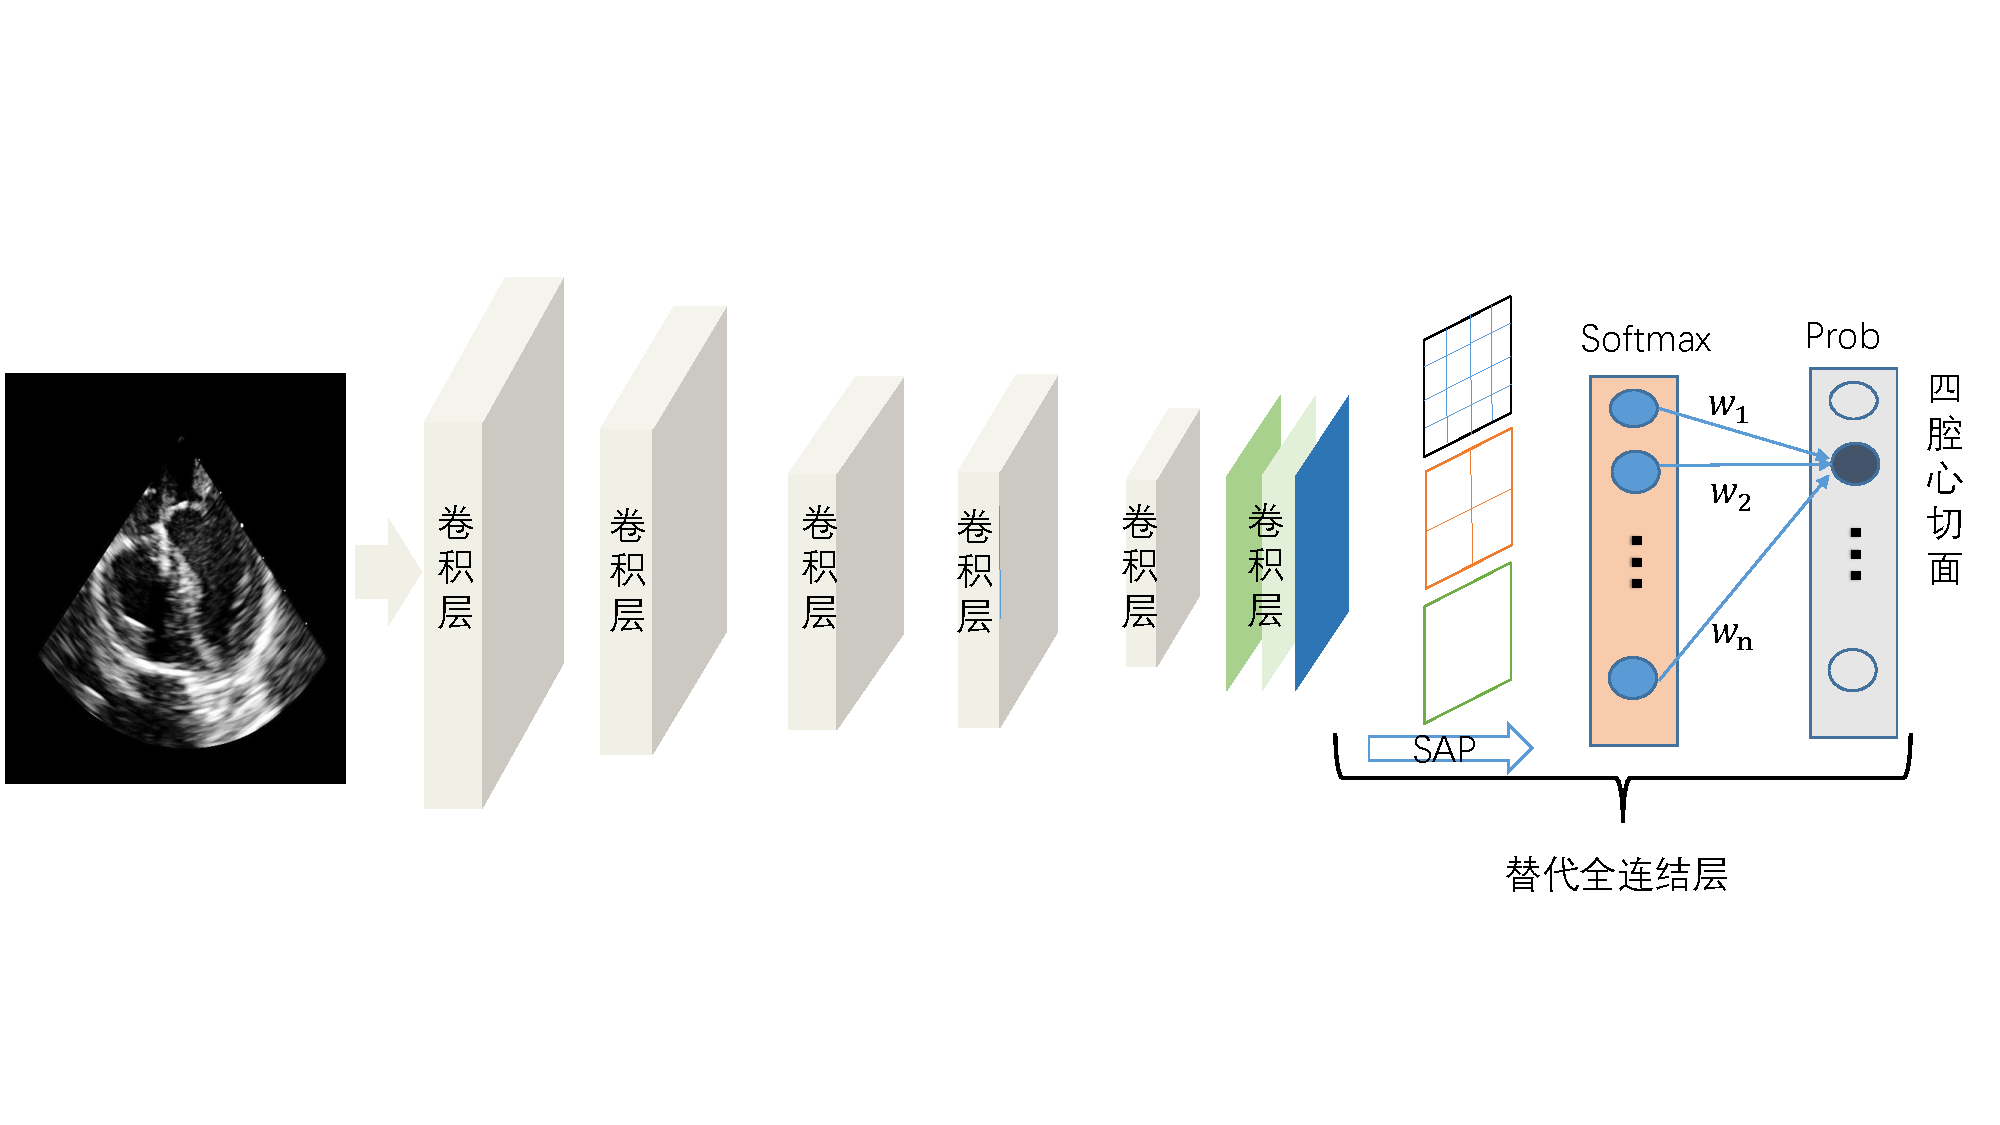
\includegraphics[trim = 30mm 0mm 30mm 0mm, clip, width=0.45\textwidth]{ch03_02}
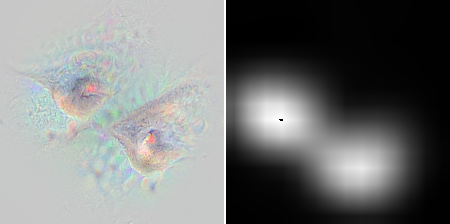
\includegraphics[width=0.85\textwidth,,height=0.2\textheight]{ch04_05}
\caption{引入类别激活图的可视化}
\label{fig:ch04_05}
\end{figure}  

实验结果见图\ref{fig:ch04_05}(a)所示,具体实验设置和图2采用的参数一致,使用提出的金字塔分解正则化技术,图\ref{fig:ch04_05}(b)为图\ref{fig:ch04_05}(a)相应的类别激活图,图\ref{fig:ch04_05}(a)结果表明与类别无关的上下文信息得到压制,但仍存在两个类别中心。

\section{本章小结}

本文针对理解深度CNN特征空间存在的问题,提出一种用于改善深度CNN分类模型的可视化方法。其中通过改善激活最大化可视化技术来产生更具有全局结构的细节、上下文信息和更自然的颜色分布的高质量图像。该方法首先对反向传播的梯度进行归一化操作,在常用正则化技术的基础上,提出使用空间金字塔分解图像不同频谱信息;为限制可视化区域,提出利用类别显著激活图技术,可以减少优化产生重复对象碎片的倾向,而倾向于产生单个中心对象以改进可视化效果。激活最大化可显示CNN在分类时关注什么。这种改进的深度可视化技术将增加我们对深层神经网络的理解,进一步提高创造更强大的深度学习算法的能力。该方法适用于基于梯度更新的可视化领域,是对网络模型整体的理解,具体各层特征怎么耦合成语义信息仍需进一步探索,深度CNN模型如何重建一个完整的类别概念,仍是一个开放性问题。
